\documentclass[11pt]{article}
\usepackage[utf8]{inputenc}
\usepackage[T1]{fontenc}
\usepackage{amsmath,amssymb,booktabs,graphicx,natbib,hyperref,geometry,xcolor}
\usepackage{microtype}
\geometry{margin=1in}
\hypersetup{colorlinks=true,linkcolor=black,citecolor=blue,urlcolor=blue}
\graphicspath{{figures/}}

\newcommand{\Pf}{\hat{P}}

\title{Statistical Power of Backtest Validation Pipelines:\\Planted-Signal Controls Against False Negatives}
\author{Hugo Marotin\thanks{Independent researcher. Code and dated campaign outputs: \url{https://github.com/hugomarotin-git/ml-papers} (folder \texttt{paper1-backtest-power}). Contact: \texttt{hugomarotin@gmail.com}.}}
\date{November 2026 --- draft v1}

\begin{document}
\maketitle

\begin{abstract}
Anti-overfitting tools for strategy research (deflated Sharpe ratios, probability of backtest overfitting, purged and combinatorial cross-validation) control the probability of adopting a strategy that has no signal. They say nothing about the probability of rejecting a strategy that has one. We measure the statistical power of a complete validation pipeline by planting a directional signal of known strength, aligned with realized outcomes, and reporting the smallest detectable signal per \emph{operating cell} (decision cadence $\times$ risk per trade) and as a function of effective sample size. On four years of hourly NASDAQ data and a proprietary-trading-firm evaluation with ruin and censoring, the same pipeline on the same data is blind in some cells and detects a 54\% directional signal in others; doubling the risk per trade turns a 70\% signal from always funded (1.000) into funded two times out of three (0.656); five of nine cells are uninterpretable because the null itself does not conclude; and the detection bar estimated from a single null draw moves by one to seven points from one draw to the next. Shortening the history shows the mechanism: the null's bar rises as paths overlap, while the planted signal's median stays put, so a weak true signal is rejected for lack of sample, not for lack of signal. A second, non-financial sequential gate on 117,429 hotel bookings reproduces the censoring, risk and sample-size patterns. We give the guards that prevent a meaningless ``detectable'' verdict and argue that any null result from a validation pipeline should be published with its measured detection floor.
\end{abstract}

\section{Introduction}
\label{sec:intro}

A validation pipeline for a trading strategy answers one question: should this strategy be deployed? Two errors are possible. A \emph{false GO} deploys a strategy that has no signal; a \emph{false NO-GO} discards a strategy that has one. The first error is heavily instrumented. Deflated Sharpe ratios \citep{bailey2014a}, the probability of backtest overfitting \citep{bailey2016}, purged and combinatorial cross-validation \citep{lopezdeprado2018}, reality checks and tests of superior predictive ability \citep{white2000,hansen2005}, raised $t$-statistic hurdles \citep{harvey2016} and random-strategy calibrations \citep{chordia2020} all bound the probability that luck passes the gate. The second error is almost never measured. Yet it is the more expensive of the two: a false GO is discovered at deployment, while a false NO-GO is never discovered at all. The strategy is dropped, the data are archived, and the pipeline that rejected it is trusted a little more.

The two errors also have different owners. A false GO is a property of the \emph{candidate}: it was lucky. A false NO-GO is a property of the \emph{pipeline}: its sample was too short, its risk budget made ruin arrive before the law of large numbers, its censoring rule silenced the cells where the answer lived, or one of its constants was simply wrong. None of these can be diagnosed from a rejection. A NO-GO verdict without a measured detection floor cannot distinguish ``no signal'' from ``this pipeline could not have seen one''.

Positive controls are the standard answer to this problem outside finance. Sequencing pipelines are calibrated with spike-in standards of known concentration \citep{jiang2011}; epidemiological estimators with synthetic outcomes injected into real data \citep{schuemie2018}; a non-inferiority trial without assay sensitivity is declared uninterpretable \citep{temple2000}. In quantitative finance the idea is very recent. \citet{zheng2026} plants a constant alpha among candidate strategies and shows that admission gates built on the deflated Sharpe ratio reject weak true signals at the cost of 93--99\% abstention; \citet{adeika2026} inject effects of known amplitude into real EEG recordings and report a detection floor per decoder. \citet{harvey2020a} calibrate Type~I and Type~II errors jointly for fund alphas and find that existing methods lack the power to detect outperforming managers.

This paper applies the positive-control idea to a complete validation pipeline rather than to a gate or a test. The pipeline under test labels hourly NASDAQ bars with a triple-barrier outcome, schedules decisions at a fixed cadence, sizes positions adaptively, and judges the resulting equity paths against the rules of a two-phase proprietary-trading-firm challenge with a fixed time budget. Its output is a lower bound on the probability of passing the challenge, compared with the 95th percentile of the same quantity under a twin null with random directions. We plant a directional signal of known strength $s$ --- the planted direction agrees with the realized label with probability $s$, so that $s=0.5$ reproduces the null exactly --- and ask: what is the smallest $s$ the pipeline sees, in which operating conditions, and why does it miss the rest?

Our contributions are the following.
\begin{enumerate}
\item An operational definition of the power of a validation pipeline: the smallest planted signal whose median verdict beats the null's bar, per operating cell (cadence $\times$ risk per trade), together with an \emph{interpretability} condition on censoring that must hold before the verdict is read (Section~\ref{sec:method}).
\item A measurement showing that this power is not a constant of the pipeline. On the same data and the same code, the smallest clearly detected signal ranges from 0.54 to 0.58, and five of nine cells cannot be read at all (Section~\ref{sec:results}, Table~\ref{tab:cells}).
\item The counter-intuitive result that a higher risk budget makes a strong true signal invisible: at two decisions per day, a 70\% signal is funded with probability 1.000 at 1\% risk and 0.656 at 2\% (Section~\ref{sec:risk}).
\item A measurement of power as a function of sample size, which isolates the mechanism of the false NO-GO: the null's bar rises as the usable history shrinks, while the signal's median does not fall (Section~\ref{sec:n}). On a single market series, sample size and regime are confounded; we report the confound rather than smoothing it over.
\item A non-financial replication: a two-phase sequential acceptance gate on a public stream of 117,429 hotel bookings reproduces the uninterpretable low-risk cells, the risk penalty on true signals, and the monotone fall of the null's bar with sample size, and shows that heavy-tailed stakes cost power without creating false positives (Section~\ref{sec:beyond}).
\item Three failure modes that produce a meaningless ``detectable'' verdict --- a saturated test grid, a wrong chance reference, and an uncensored null --- and the guards that close them (Section~\ref{sec:guards}).
\end{enumerate}

Every campaign result in this paper is read from a dated output file produced by the released code; no number was adjusted after the grid was fixed, and the one deviation from the pre-registered grid (Section~\ref{sec:n}) is stated with its reason.

\section{Related Work}
\label{sec:related}
% related_work.tex — Section 2 (Related Work), included from main.tex via % related_work.tex — Section 2 (Related Work), included from main.tex via % related_work.tex — Section 2 (Related Work), included from main.tex via \input{related_work}.
% Source: knowledge/50-publications/paper-1-biblio.md, section "Related Work (ébauche en anglais)".
% Citations use natbib (\citet / \citep); keys live in references.bib.

\paragraph{Backtest overfitting and the false-positive toolkit.}
A large literature protects strategy research against selection luck. \citet{bailey2012,bailey2014a} derive the probabilistic Sharpe ratio and the expected maximum of $N$ Sharpe ratios under the null, and deflate reported Sharpe ratios accordingly; \citet{bailey2014b,bailey2016} bound the minimum backtest length and estimate the probability of backtest overfitting through combinatorially symmetric cross-validation, later extended to purged and combinatorial cross-validation \citep{lopezdeprado2018}. In the multiple-testing tradition, \citet{white2000} and \citet{hansen2005} test the best of many models against the universe it was drawn from, \citet{harvey2016} raise the factor hurdle to $t > 3$, \citet{harvey2015} derive non-linear Sharpe haircuts, and \citet{chordia2020} calibrate thresholds on two million random strategies. \citet{bajgrowicz2012} and \citet{novymarx2015} apply the same logic to technical rules and combined signals. All of these instruments control the probability of adopting a strategy that has no signal. None of them reports the probability of rejecting a strategy that has one.

\paragraph{Power and missed discoveries.}
The false-negative side has been studied on a different object. \citet{harvey2020a} calibrate Type I and Type II errors jointly for the cross-section of fund alphas and conclude that existing methods lack power to detect outperforming managers; \citet{andrikogiannopoulou2019} simulate funds with known alphas and show that the false-discovery-rate procedure of \citet{barras2010} misclassifies up to 65\% of economically large alphas as zero. \citet{harvey2020b} compare the size and power of multiple-testing corrections by simulation, and \citet{inoue2005} show that out-of-sample tests sacrifice power relative to in-sample tests of the same hypothesis. These studies treat power as a property of a test applied to a distribution of effects, not of an operating pipeline with a decision frequency, a risk budget and a finite horizon.

\paragraph{Planted signals as positive controls.}
Validating a pipeline by injecting a known effect is standard outside finance: spike-in standards of known concentration measure the sensitivity of sequencing pipelines \citep{jiang2011}; synthetic positive controls, obtained by injecting simulated outcomes into real observational data, calibrate confidence intervals of epidemiological estimators \citep{schuemie2018}; active-control trials are uninterpretable without assay sensitivity \citep{temple2000}; randomization tests check that an explanation method reacts to the model it claims to explain \citep{adebayo2018}. Closest to our design, \citet{adeika2026} inject class-dependent effects of known amplitude into real EEG recordings and report a measured \emph{detection floor} per decoder, recommending that every null result be accompanied by one. The idea reached quantitative finance only recently. \citet{zheng2026} plants a constant alpha among candidate strategies and measures the adoption rate of admission gates built on the deflated Sharpe ratio against a random-admission control: gates remove false discoveries for weak signals at the cost of 93--99\% abstention, and criteria computed on absolute returns silently reject every true signal. \citet{liu2026} and \citet{qu2026} use planted-signal worlds to measure the size and power of LLM research agents and the admission delay of an anytime-valid referee. \citet{santoni2026} and \citet{gencay2026} evaluate composite robustness scores and search-aware deflation, again on the false-positive side.

\paragraph{Effective sample size, sequential stopping and censoring.}
Overlapping observations shrink the effective sample far below the nominal count \citep{hansen1980,boudoukh2008,lo2002}, and minimum-sample-size rules for prediction models are stated per event, not per row \citep{riley2019}. Sequential tests have a power function and an expected stopping time \citep{wald1945,doerks2026}, repeated looks inflate size \citep{armitage1969,lan1983,johari2022}, and a fixed fraction at risk determines the probability of ruin \citep{kelly1956,peters2019}. Incomplete observations are the domain of survival analysis \citep{kaplan1958}, and conditioning on survivors manufactures performance \citep{brown1992}.

\paragraph{Our contribution}
connects these strands: we treat the validation pipeline itself as the object whose power is measured, plant a signal of known directional strength aligned with realized outcomes, and report the smallest detectable signal per operating cell (decision cadence $\times$ risk per trade) and as a function of effective sample size, declaring a cell uninterpretable when the time budget censors the null or the signal. Unlike \citet{zheng2026}, we vary the operating cell rather than the gate, and find that the same pipeline on the same data is blind in some cells and detects a 54\% signal in others, and that a higher risk budget can make a strong true signal invisible.

% ---------------------------------------------------------------------------
% Citation check (2026-11-09): every \citet/\citep key above was matched against
% references.bib. Unresolved citations: none.
% ---------------------------------------------------------------------------
.
% Source: knowledge/50-publications/paper-1-biblio.md, section "Related Work (ébauche en anglais)".
% Citations use natbib (\citet / \citep); keys live in references.bib.

\paragraph{Backtest overfitting and the false-positive toolkit.}
A large literature protects strategy research against selection luck. \citet{bailey2012,bailey2014a} derive the probabilistic Sharpe ratio and the expected maximum of $N$ Sharpe ratios under the null, and deflate reported Sharpe ratios accordingly; \citet{bailey2014b,bailey2016} bound the minimum backtest length and estimate the probability of backtest overfitting through combinatorially symmetric cross-validation, later extended to purged and combinatorial cross-validation \citep{lopezdeprado2018}. In the multiple-testing tradition, \citet{white2000} and \citet{hansen2005} test the best of many models against the universe it was drawn from, \citet{harvey2016} raise the factor hurdle to $t > 3$, \citet{harvey2015} derive non-linear Sharpe haircuts, and \citet{chordia2020} calibrate thresholds on two million random strategies. \citet{bajgrowicz2012} and \citet{novymarx2015} apply the same logic to technical rules and combined signals. All of these instruments control the probability of adopting a strategy that has no signal. None of them reports the probability of rejecting a strategy that has one.

\paragraph{Power and missed discoveries.}
The false-negative side has been studied on a different object. \citet{harvey2020a} calibrate Type I and Type II errors jointly for the cross-section of fund alphas and conclude that existing methods lack power to detect outperforming managers; \citet{andrikogiannopoulou2019} simulate funds with known alphas and show that the false-discovery-rate procedure of \citet{barras2010} misclassifies up to 65\% of economically large alphas as zero. \citet{harvey2020b} compare the size and power of multiple-testing corrections by simulation, and \citet{inoue2005} show that out-of-sample tests sacrifice power relative to in-sample tests of the same hypothesis. These studies treat power as a property of a test applied to a distribution of effects, not of an operating pipeline with a decision frequency, a risk budget and a finite horizon.

\paragraph{Planted signals as positive controls.}
Validating a pipeline by injecting a known effect is standard outside finance: spike-in standards of known concentration measure the sensitivity of sequencing pipelines \citep{jiang2011}; synthetic positive controls, obtained by injecting simulated outcomes into real observational data, calibrate confidence intervals of epidemiological estimators \citep{schuemie2018}; active-control trials are uninterpretable without assay sensitivity \citep{temple2000}; randomization tests check that an explanation method reacts to the model it claims to explain \citep{adebayo2018}. Closest to our design, \citet{adeika2026} inject class-dependent effects of known amplitude into real EEG recordings and report a measured \emph{detection floor} per decoder, recommending that every null result be accompanied by one. The idea reached quantitative finance only recently. \citet{zheng2026} plants a constant alpha among candidate strategies and measures the adoption rate of admission gates built on the deflated Sharpe ratio against a random-admission control: gates remove false discoveries for weak signals at the cost of 93--99\% abstention, and criteria computed on absolute returns silently reject every true signal. \citet{liu2026} and \citet{qu2026} use planted-signal worlds to measure the size and power of LLM research agents and the admission delay of an anytime-valid referee. \citet{santoni2026} and \citet{gencay2026} evaluate composite robustness scores and search-aware deflation, again on the false-positive side.

\paragraph{Effective sample size, sequential stopping and censoring.}
Overlapping observations shrink the effective sample far below the nominal count \citep{hansen1980,boudoukh2008,lo2002}, and minimum-sample-size rules for prediction models are stated per event, not per row \citep{riley2019}. Sequential tests have a power function and an expected stopping time \citep{wald1945,doerks2026}, repeated looks inflate size \citep{armitage1969,lan1983,johari2022}, and a fixed fraction at risk determines the probability of ruin \citep{kelly1956,peters2019}. Incomplete observations are the domain of survival analysis \citep{kaplan1958}, and conditioning on survivors manufactures performance \citep{brown1992}.

\paragraph{Our contribution}
connects these strands: we treat the validation pipeline itself as the object whose power is measured, plant a signal of known directional strength aligned with realized outcomes, and report the smallest detectable signal per operating cell (decision cadence $\times$ risk per trade) and as a function of effective sample size, declaring a cell uninterpretable when the time budget censors the null or the signal. Unlike \citet{zheng2026}, we vary the operating cell rather than the gate, and find that the same pipeline on the same data is blind in some cells and detects a 54\% signal in others, and that a higher risk budget can make a strong true signal invisible.

% ---------------------------------------------------------------------------
% Citation check (2026-11-09): every \citet/\citep key above was matched against
% references.bib. Unresolved citations: none.
% ---------------------------------------------------------------------------
.
% Source: knowledge/50-publications/paper-1-biblio.md, section "Related Work (ébauche en anglais)".
% Citations use natbib (\citet / \citep); keys live in references.bib.

\paragraph{Backtest overfitting and the false-positive toolkit.}
A large literature protects strategy research against selection luck. \citet{bailey2012,bailey2014a} derive the probabilistic Sharpe ratio and the expected maximum of $N$ Sharpe ratios under the null, and deflate reported Sharpe ratios accordingly; \citet{bailey2014b,bailey2016} bound the minimum backtest length and estimate the probability of backtest overfitting through combinatorially symmetric cross-validation, later extended to purged and combinatorial cross-validation \citep{lopezdeprado2018}. In the multiple-testing tradition, \citet{white2000} and \citet{hansen2005} test the best of many models against the universe it was drawn from, \citet{harvey2016} raise the factor hurdle to $t > 3$, \citet{harvey2015} derive non-linear Sharpe haircuts, and \citet{chordia2020} calibrate thresholds on two million random strategies. \citet{bajgrowicz2012} and \citet{novymarx2015} apply the same logic to technical rules and combined signals. All of these instruments control the probability of adopting a strategy that has no signal. None of them reports the probability of rejecting a strategy that has one.

\paragraph{Power and missed discoveries.}
The false-negative side has been studied on a different object. \citet{harvey2020a} calibrate Type I and Type II errors jointly for the cross-section of fund alphas and conclude that existing methods lack power to detect outperforming managers; \citet{andrikogiannopoulou2019} simulate funds with known alphas and show that the false-discovery-rate procedure of \citet{barras2010} misclassifies up to 65\% of economically large alphas as zero. \citet{harvey2020b} compare the size and power of multiple-testing corrections by simulation, and \citet{inoue2005} show that out-of-sample tests sacrifice power relative to in-sample tests of the same hypothesis. These studies treat power as a property of a test applied to a distribution of effects, not of an operating pipeline with a decision frequency, a risk budget and a finite horizon.

\paragraph{Planted signals as positive controls.}
Validating a pipeline by injecting a known effect is standard outside finance: spike-in standards of known concentration measure the sensitivity of sequencing pipelines \citep{jiang2011}; synthetic positive controls, obtained by injecting simulated outcomes into real observational data, calibrate confidence intervals of epidemiological estimators \citep{schuemie2018}; active-control trials are uninterpretable without assay sensitivity \citep{temple2000}; randomization tests check that an explanation method reacts to the model it claims to explain \citep{adebayo2018}. Closest to our design, \citet{adeika2026} inject class-dependent effects of known amplitude into real EEG recordings and report a measured \emph{detection floor} per decoder, recommending that every null result be accompanied by one. The idea reached quantitative finance only recently. \citet{zheng2026} plants a constant alpha among candidate strategies and measures the adoption rate of admission gates built on the deflated Sharpe ratio against a random-admission control: gates remove false discoveries for weak signals at the cost of 93--99\% abstention, and criteria computed on absolute returns silently reject every true signal. \citet{liu2026} and \citet{qu2026} use planted-signal worlds to measure the size and power of LLM research agents and the admission delay of an anytime-valid referee. \citet{santoni2026} and \citet{gencay2026} evaluate composite robustness scores and search-aware deflation, again on the false-positive side.

\paragraph{Effective sample size, sequential stopping and censoring.}
Overlapping observations shrink the effective sample far below the nominal count \citep{hansen1980,boudoukh2008,lo2002}, and minimum-sample-size rules for prediction models are stated per event, not per row \citep{riley2019}. Sequential tests have a power function and an expected stopping time \citep{wald1945,doerks2026}, repeated looks inflate size \citep{armitage1969,lan1983,johari2022}, and a fixed fraction at risk determines the probability of ruin \citep{kelly1956,peters2019}. Incomplete observations are the domain of survival analysis \citep{kaplan1958}, and conditioning on survivors manufactures performance \citep{brown1992}.

\paragraph{Our contribution}
connects these strands: we treat the validation pipeline itself as the object whose power is measured, plant a signal of known directional strength aligned with realized outcomes, and report the smallest detectable signal per operating cell (decision cadence $\times$ risk per trade) and as a function of effective sample size, declaring a cell uninterpretable when the time budget censors the null or the signal. Unlike \citet{zheng2026}, we vary the operating cell rather than the gate, and find that the same pipeline on the same data is blind in some cells and detects a 54\% signal in others, and that a higher risk budget can make a strong true signal invisible.

% ---------------------------------------------------------------------------
% Citation check (2026-11-09): every \citet/\citep key above was matched against
% references.bib. Unresolved citations: none.
% ---------------------------------------------------------------------------


\section{The Validation Pipeline Under Test}
\label{sec:pipeline}

The object whose power we measure is a full pipeline, not a statistic. We describe each stage in general terms, then give the instantiation used in the experiments. All constants below were fixed before the campaigns reported here were run; none was tuned on their results.

\paragraph{Data.}
Hourly bars of a NASDAQ-100 CFD from a proprietary-trading-firm feed, development window 2021-01-22 to 2024-12-31: 23,312 bars, 1,020 trading days in the firm's day convention (18:00 to 16:00 New York, crossing midnight), 17,177 labelled candidate bars. A later hold-out period is sealed and was never read for this work; the paper therefore makes no claim about the existence of a real signal in this market, only about what the pipeline can see.

\paragraph{Labels.}
Each candidate bar $t$ receives a triple-barrier label \citep{lopezdeprado2018}: a trade entered at the open of $t+1$ with symmetric barriers at $\pm 1.5$ ATR (ATR frozen at $t$) and a horizon of six bars is classified by which event comes first: upper barrier (28.6\% of labels), lower barrier (29.7\%), both barriers inside the same hourly bar (2.0\%, counted as a loss for either direction since the order is unknown), or timeout (39.7\%, closed at market). The seven bars must be contiguous; candidates whose horizon crosses a market close are discarded. The reward-to-risk ratio of a barrier-decided trade is therefore 1:1 by construction, and a coin-flip direction has an expected payoff of $-P(\text{both}) = -0.02$ barrier distances per label, not zero.

\paragraph{Decision calendar and cadence.}
A calendar draws candidate instants at a fixed cadence $c \in \{0.5, 1, 2\}$ decisions per trading day, spread within the day rather than pinned to the open, from a seed fixed once per campaign. All planted signals and the null of a cell share the same calendar: only the direction differs.

\paragraph{Scheduler.}
One position at a time. Candidates that arrive while a position is open are dropped. The scheduler is greedy in time, which is the only policy a trader can execute without knowing the future, and it runs before any sizing so that every configuration plays exactly the same sequence of trades.

\paragraph{Sizing.}
Position size is set so that a stop-out loses a fraction $r \cdot m$ of the initial capital, with base risk $r \in \{0.5\%, 1\%, 2\%\}$ and an adaptive multiplier $m \in [0.25, 1.25]$ updated at the close of each trading day from the day's realized result: $+0.25$ after a winning day, halved after three consecutive losing days, reset at phase change. Updates happen at the day boundary, so $m$ can only affect positions opened afterwards. The multiplier was calibrated on the null before this work and is not varied here.

\paragraph{Evaluation rules.}
The equity path is judged against a two-phase challenge on a 50,000 account: phase~1 requires $+10\%$ and phase~2 $+5\%$, each requiring at least four trading days and each lost if equity falls $10\%$ below the phase's starting capital or more than a fixed 2,500 ($5\%$ of the initial capital) below the balance at the daily reset (17:00 New York, server midnight). Phase~2 restarts at the initial capital. Targets are judged on closed balance, floors on equity including open positions. Transaction costs are not modelled.

\paragraph{Paths, budget and censoring.}
A path starts at every third trade of the executed sequence and is given a budget of $B = 250$ trading days (one year) to conclude. Only starts with the full budget ahead of them are played, so a history of $n$ trading days yields starts on its first $n - B$ days. A path ends \emph{funded} (both phases passed), \emph{busted} (a floor touched) or \emph{censored} (budget exhausted). The pipeline reports the lower bound
\begin{equation}
\Pf = \frac{\#\text{funded}}{\#\text{paths}},
\label{eq:lb}
\end{equation}
which counts censored paths as failures, together with the censoring rate.

\paragraph{The null and its bar.}
The null is a \emph{twin}: same instrument, same labels and barriers, same calendar, same scheduler, same sizing, same rules; only the direction of each trade is a coin flip. It is replayed with 60 direction seeds, and the pipeline's bar for a cell is the 95th percentile of $\Pf$ across those replications. A candidate is declared to beat the null when its $\Pf$ exceeds this bar.

\section{Planted-Signal Controls}
\label{sec:method}

\paragraph{The planted signal.}
For a signal strength $s \in [0.5, 1]$, the planted decider looks at the realized label of each scheduled candidate. If the label is directional (upper or lower barrier first), it takes the winning direction with probability $s$ and the losing one with probability $1-s$; if the label is non-directional (both or timeout), it flips a coin, since no direction wins. The realized directional accuracy of the planted decider is thus $s$ by construction, up to sampling noise, and $s = 0.5$ reproduces the twin null exactly: the proof suite checks that at $s = 0.5$ the number of trades and the counts of discarded candidates coincide with the null's. The injector reads the future on purpose; it is a calibration instrument for the \emph{evaluation} chain and has no place in a decider. It does not test whether a learner can find a signal in features; that is a separate positive control.

\paragraph{The measurement.}
An operating cell is a pair (cadence $c$, base risk $r$). In each cell, every strength in a pre-registered grid is played through the full pipeline with the 60 direction seeds, producing a distribution of $\Pf$ per strength. We report the median $\Pf_{50}(s)$ and define the \emph{margin} $\Delta(s) = \Pf_{50}(s) - \text{bar}$, where the bar is the null's 95th percentile in the same cell, from the same calendar and the same seeds. A strength is \emph{detectable} when $\Delta(s) > 0$; the \emph{detection floor} of a cell is the smallest detectable strength on the grid. We also report a \emph{clear} floor, defined in the next paragraph, and the floors quoted in the text are clear floors unless stated otherwise.

\paragraph{Interpretability.}
A cell is \emph{interpretable} only if the median censoring rate is at most 10\% both for the null and for the planted signal, a threshold fixed before the campaigns. When the null does not conclude, its lower bound~\eqref{eq:lb} collapses towards zero whatever the data say, and the bar becomes trivially easy to beat; when the signal does not conclude, its $\Pf$ is capped by censoring, not by skill. In both cases ``detectable'' is a statement about the budget, not about the signal. The guard is enforced in code: an uninterpretable cell returns no detection floor.

\paragraph{Noise of the bar.}
The bar is itself an estimate from 60 draws. We re-draw the null with two further sets of 60 seeds and report the standard deviation of the bar across the three draws. A strength is detected \emph{clearly} when its margin exceeds this standard deviation; otherwise its detection depends on which null sample happened to be drawn.

\paragraph{Pre-registration.}
Grids, cells, seeds and reading criteria were written down before each campaign ran and are reproduced in the released repository. Campaign~A measures the detection floor on strengths $\{0.52, 0.54, 0.55, 0.56, 0.58, 0.62, 0.70\}$ plus the null in the nine cells (4,320 pipeline runs on the full 1,020-day history, 57 minutes on nine cores). Campaigns~B$_1$ and B$_2$ re-draw the null (seeds 60--119 and 120--179) with strengths 0.55 and 0.58. Campaign~C shortens the development window to its most recent 1, 2 and 3 years and replays two cells.

\section{Results on the Financial Pipeline}
\label{sec:results}

\subsection{Power by operating cell}
\label{sec:cells}

Table~\ref{tab:cells} and Figure~\ref{fig:cells} give the full campaign~A. Four cells are interpretable. In them the clear detection floor is 0.54 at two decisions per day (both at 1\% and 2\% risk), 0.56 at one decision per day and 2\% risk, and 0.58 at half a decision per day and 2\% risk; with any positive margin accepted, the last two floors drop to 0.55 and 0.56. A 0.52 signal is drowned in every interpretable cell. The same pipeline, on the same four years of data, thus needs a directional accuracy anywhere between 54\% and 58\% before it can tell a real signal from a coin flip, and that number depends on how often the strategy trades and how much it risks, not on the strategy.

\begin{table}[t]
\centering\small
\caption{Campaign A. Per cell: the null's bar ($p_{95}$ of $\Pf$ over 60 direction seeds), its standard deviation over three independent null draws (campaigns A, B$_1$, B$_2$), the null's median censoring rate, the median $\Pf$ of three planted strengths, and the smallest strength on the grid whose margin is positive (\emph{any}) or exceeds the bar's standard deviation (\emph{clear}). A cell is uninterpretable when the median censoring of the null or of a planted signal exceeds 10\%; in this campaign the null's censoring is always the binding one.}
\label{tab:cells}
\footnotesize
\begin{tabular}{rrrrrrrrrr}
\toprule
Cadence & Risk & Null bar & Bar s.d. & Null cens. & \multicolumn{3}{c}{Signal median $\hat P$} & \multicolumn{2}{c}{Smallest detectable} \\
\cmidrule(lr){6-8}\cmidrule(lr){9-10}
(dec./day) & (\%) & ($p_{95}$) & (3 draws) & (median) & $s=0.55$ & $s=0.58$ & $s=0.70$ & any & clear \\
\midrule
0.5 & 0.5 & 0.001 & 0.000 & 0.957 & 0.000 & 0.008 & 0.626 & \multicolumn{2}{c}{\emph{uninterpretable}} \\
0.5 & 1 & 0.255 & 0.069 & 0.406 & 0.287 & 0.441 & 1.000 & \multicolumn{2}{c}{\emph{uninterpretable}} \\
0.5 & 2 & 0.444 & 0.056 & 0.000 & 0.398 & 0.555 & 0.917 & 0.56 & 0.58 \\
1 & 0.5 & 0.082 & 0.016 & 0.798 & 0.101 & 0.327 & 1.000 & \multicolumn{2}{c}{\emph{uninterpretable}} \\
1 & 1 & 0.441 & 0.029 & 0.150 & 0.500 & 0.763 & 1.000 & \multicolumn{2}{c}{\emph{uninterpretable}} \\
1 & 2 & 0.401 & 0.034 & 0.000 & 0.430 & 0.580 & 0.926 & 0.55 & 0.56 \\
2 & 0.5 & 0.203 & 0.027 & 0.493 & 0.379 & 0.700 & 1.000 & \multicolumn{2}{c}{\emph{uninterpretable}} \\
2 & 1 & 0.432 & 0.038 & 0.012 & 0.597 & 0.804 & 1.000 & 0.54 & 0.54 \\
2 & 2 & 0.194 & 0.007 & 0.000 & 0.228 & 0.315 & 0.656 & 0.54 & 0.54 \\
\bottomrule
\end{tabular}

\end{table}

\begin{figure}[t]
\centering
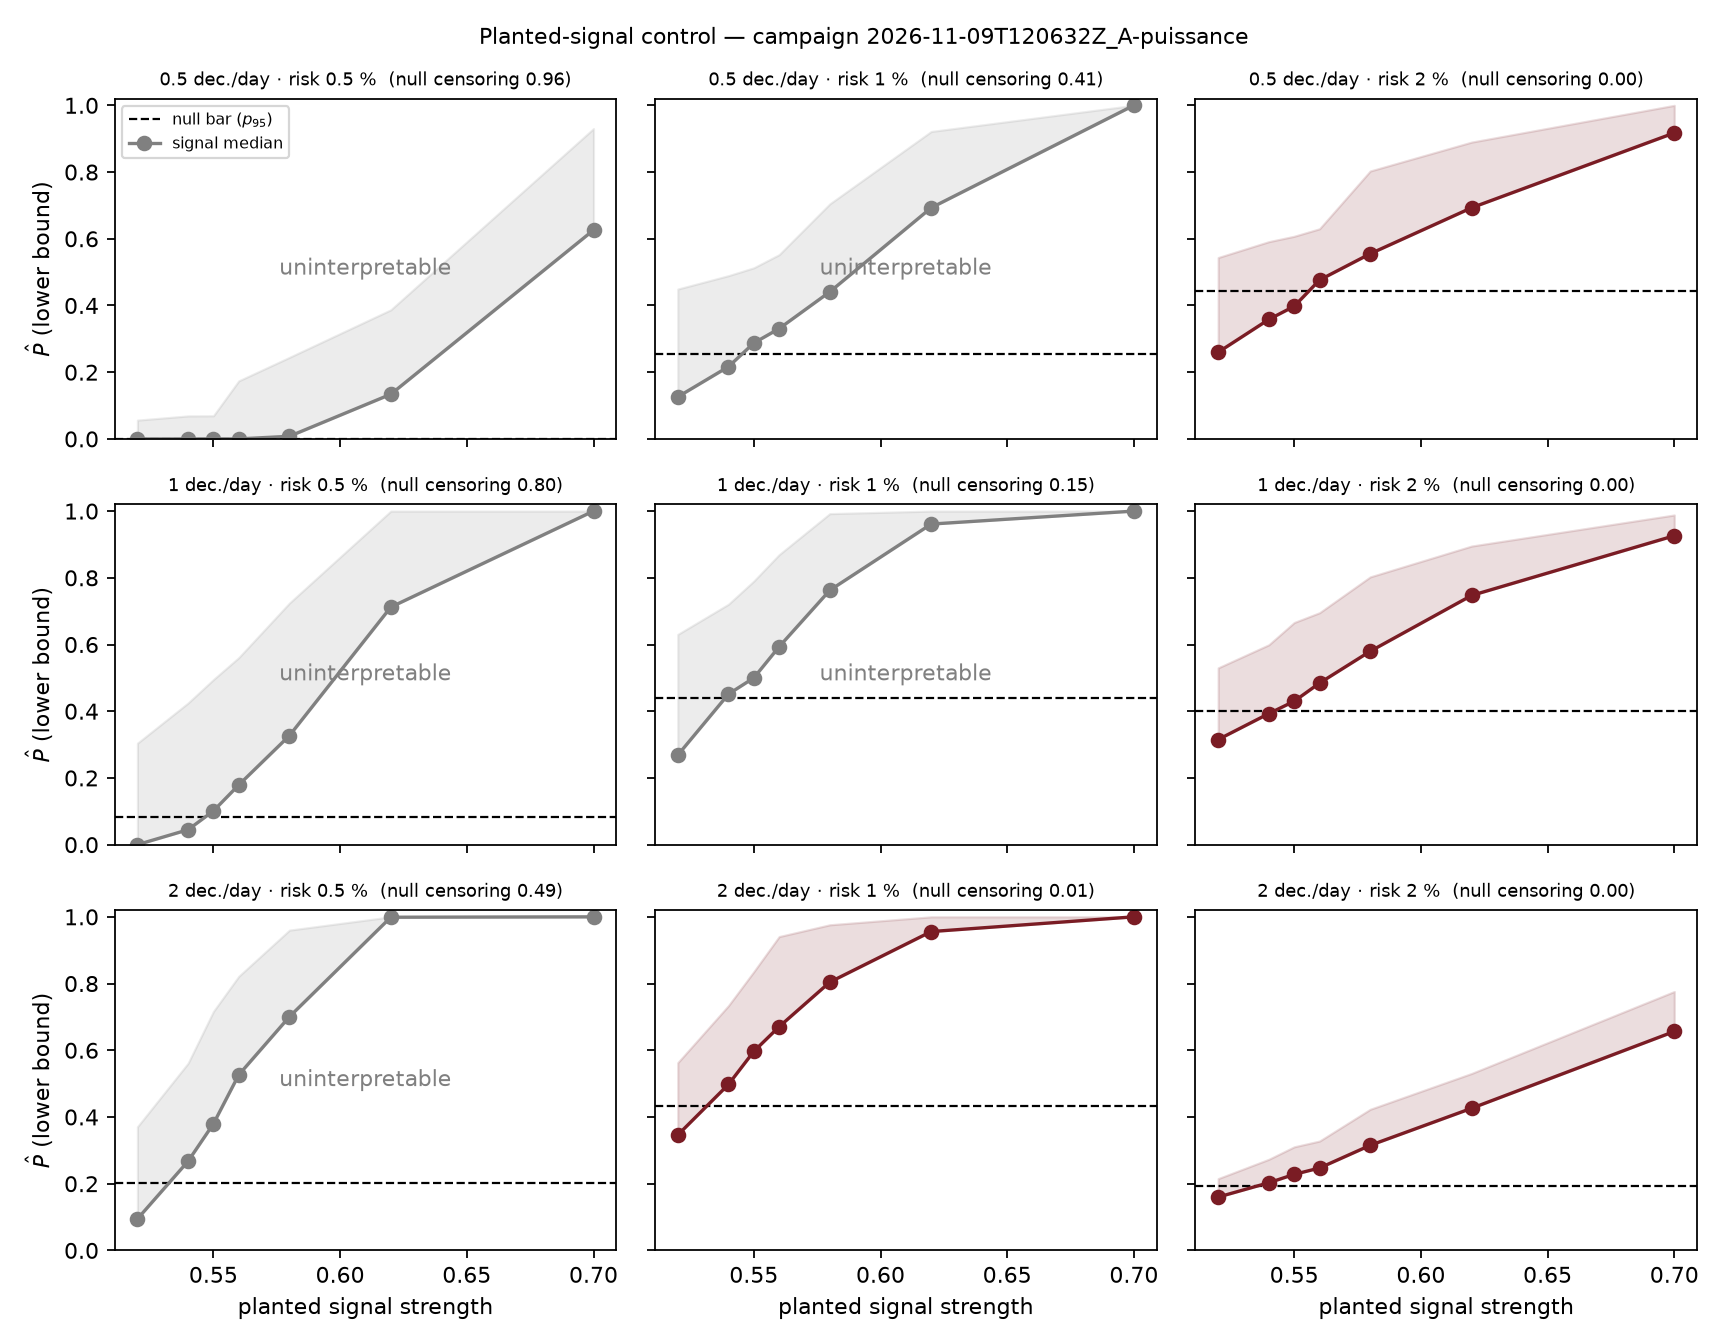
\includegraphics[width=\textwidth]{fig1_cellules}
\caption{Campaign A, nine operating cells (rows: decisions per day; columns: risk per trade). Dashed line: the null's bar. Solid line: median $\Pf$ of the planted signal as a function of its strength; band: median to 95th percentile over 60 seeds. Grey cells are uninterpretable (null censoring above 10\%). In the grey cells the curves rise steeply, yet nothing can be read from them.}
\label{fig:cells}
\end{figure}

The margin between two neighbouring strengths is of the order of the bar's noise. At one decision per day and 2\% risk, strength 0.55 beats the bar by 0.029 while the bar's standard deviation across draws is 0.034; strength 0.56 beats it by 0.083. A single null sample would have declared 0.55 detectable or drowned depending on the draw. At two decisions per day and 2\% risk the floor of 0.54 is formally clear (margin 0.009 against 0.007) but should be read as borderline. The honest floor is therefore an interval of about two points of accuracy, and anyone quoting a single number from one null draw is quoting the draw.

\subsection{Noise of the null bar}
\label{sec:noise}

The bar's standard deviation over three draws of 60 seeds is 0.069 at half a decision per day and 1\% risk, 0.056 at half a decision and 2\%, 0.038 at two decisions and 1\%, 0.034 at one decision and 2\%, and 0.007 at two decisions and 2\% (Table~\ref{tab:cells}, fourth column). These are large relative to the margins that decide a verdict: a strategy whose $\Pf$ exceeds the bar by three points at one decision per day has not been shown to beat the null. The noise is largest where paths are fewest and most dependent, which is also where the pipeline is most often used in practice: low cadence, moderate risk.

\subsection{Risk makes a true signal invisible}
\label{sec:risk}

At two decisions per day, a planted signal of strength 0.70 is funded with median probability 1.000 at 1\% risk and 0.656 at 2\%. Strength 0.62 gives 0.956 against 0.426; strength 0.58 gives 0.804 against 0.315. At one decision per day, strength 0.58 gives 0.763 at 1\% (a cell that is itself uninterpretable) against 0.580 at 2\%. Doubling the risk per trade removes between a third and two thirds of the probability that a genuinely strong strategy passes the evaluation.

The mechanism is that ruin is a first-passage event. With a 10\% floor and a stop of about 2\% of capital, five consecutive full-size losses end the path; at an accuracy of 70\% the probability of five straight losses on any given run of five trades is $0.3^5 \approx 0.24\%$, but a path of several hundred trades offers hundreds of such runs, and the daily floor adds a second barrier. The law of large numbers that makes a 70\% strategy profitable needs more trades than a 2\% risk budget allows it to survive. The pipeline is not wrong to reject such a configuration --- a real account would also bust --- but a researcher who tests a candidate only at 2\% risk and concludes ``no signal'' has drawn the wrong conclusion from a correct verdict.

\subsection{Power as a function of sample size}
\label{sec:n}

Campaign~C replays two interpretable cells fixed in the pre-registered grid, one decision per day at 2\% risk and two decisions per day at 1\% risk, on the development window shortened to its most recent 1.5, 2 and 3 years, with the full window (1,020 trading days) taken from campaign~A. Table~\ref{tab:n} and Figure~\ref{fig:n} report the null's bar and the margin of three strengths against the number of \emph{usable} trading days $n - B$: a window of $n$ days with a budget of $B = 250$ days can start a complete path only on its first $n - B$ days.

\begin{table}[t]
\centering\small
\caption{Campaign C. Null bar and margins $\Delta(s) = \Pf_{50}(s) - \text{bar}$ as a function of the usable history (window length minus the one-year budget). Bold: positive margin. The pre-registered 1-year window yields zero usable days and is omitted (see text).}
\label{tab:n}
\begin{tabular}{llrrrr}
\toprule
\multicolumn{2}{l}{Usable trading days $n - B$} & 125 & 250 & 500 & 770 \\
\multicolumn{2}{l}{Development window (years)} & 1.5 & 2 & 3 & 4 (full) \\
\midrule
\multicolumn{2}{l}{\emph{1 dec./day, risk 2\,\%}} & 0.668 & 0.595 & 0.419 & 0.401 \\
& $s=0.55$ & -0.263 & -0.137 & -0.003 & \textbf{+0.029} \\
& $s=0.58$ & -0.049 & \textbf{+0.048} & \textbf{+0.144} & \textbf{+0.179} \\
& $s=0.62$ & \textbf{+0.070} & \textbf{+0.185} & \textbf{+0.305} & \textbf{+0.346} \\
\multicolumn{2}{l}{\emph{2 dec./day, risk 1\,\%}} & 0.864 & 0.418 & 0.606 & 0.432 \\
& $s=0.55$ & -0.175 & \textbf{+0.011} & -0.056 & \textbf{+0.165} \\
& $s=0.58$ & \textbf{+0.083} & \textbf{+0.353} & \textbf{+0.166} & \textbf{+0.372} \\
& $s=0.62$ & \textbf{+0.136} & \textbf{+0.526} & \textbf{+0.348} & \textbf{+0.524} \\
\bottomrule
\end{tabular}

\end{table}

\begin{figure}[t]
\centering
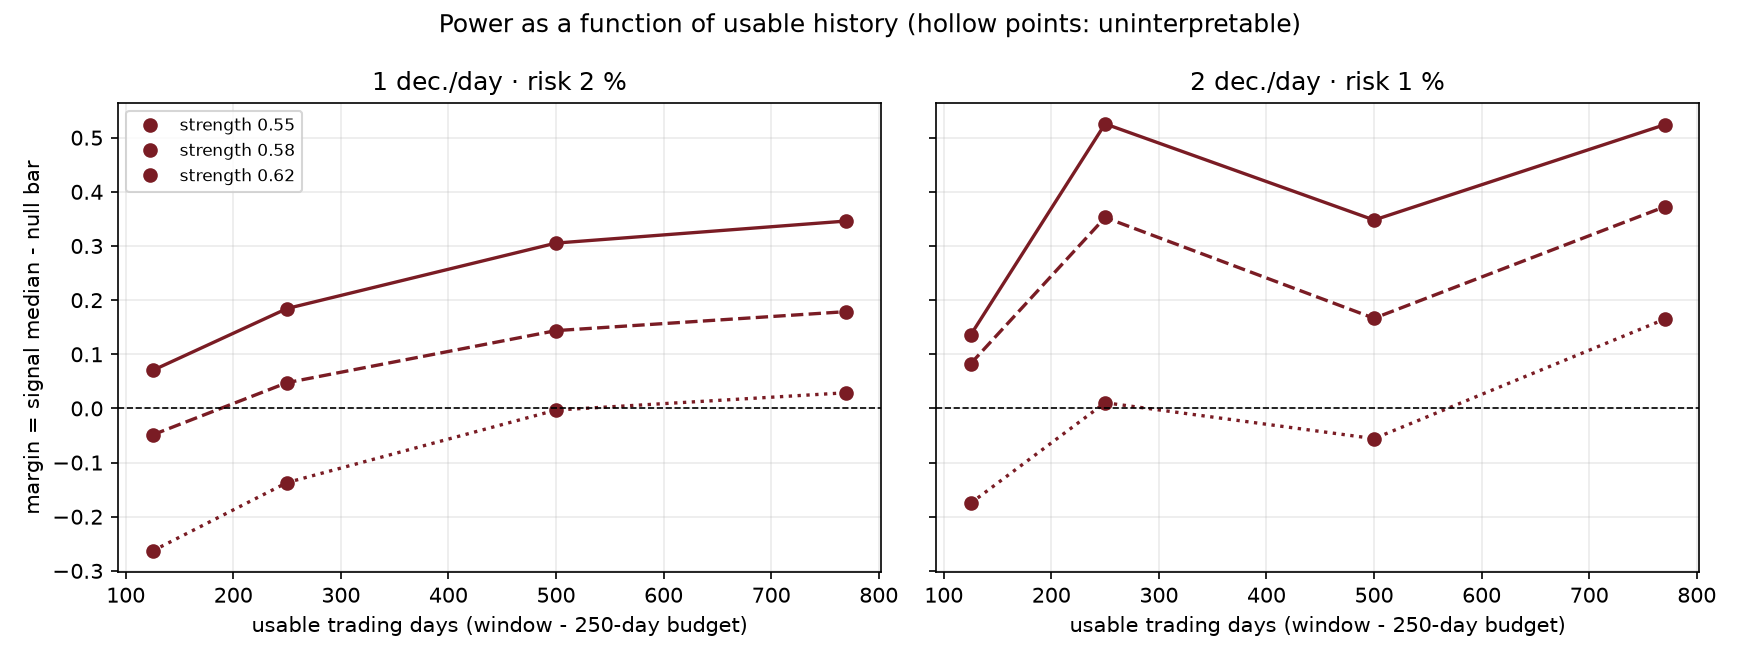
\includegraphics[width=\textwidth]{fig3_puissance_n}
\caption{Campaign C. Margin of three planted strengths as a function of the usable history, for the two cells replayed. Left: one decision per day, 2\% risk, a clean monotone power curve. Right: two decisions per day, 1\% risk, where the regime of the start dates dominates the sample size.}
\label{fig:n}
\end{figure}

One deviation from the pre-registered grid was decided after the 1-year run and before any result of the 2- and 3-year runs was read. The pre-registered 1-year window is structurally empty: 250 days of history with a 250-day budget leave a single start per seed, so $\Pf$ is 0 or 1 and the null's 95th percentile is 1.000 by construction. This is not a bug of the pipeline but a property of any sequential evaluation with a time budget: the effective sample is the history \emph{minus} the budget. We replaced the point by a 1.5-year window. A second point is not a deviation but a limit of the design: the four windows are nested from the end of the development period (start dates 2023-07, 2023-01, 2022-02, 2021-01), so a longer window adds \emph{earlier} data, and sample size is confounded with market regime. We did not attempt to deconfound them.

At one decision per day and 2\% risk, the result is a clean power curve. The null's bar falls from 0.668 to 0.595, 0.419 and 0.401 as the usable history grows from 125 to 770 days, while the medians of the planted signals stay within eight points of each other. Strength 0.62 is detected from 125 usable days, strength 0.58 from 250, strength 0.55 only at 770. Three strengths, three sample sizes at which the pipeline starts to see them: this is the false NO-GO by lack of history, measured.

At two decisions per day and 1\% risk, the regime dominates. The bar reads 0.864, 0.418, 0.606 and 0.432 as the window grows: it is not monotone, because each window adds a different stretch of history, and the coin-flip decider passes far more often when the starts are confined to the second half of 2023 (1.5-year window) than when the first half of 2023 is included (2-year window). Strength 0.55 is detected at 250 usable days (barely, by 0.011) and at 770, and drowned at 125 and 500. On a single market series the null's bar is not a constant of the pipeline; it moves with the window by up to 0.45, and the detection floor moves with it. We report this as it is. It strengthens rather than weakens the paper's point: a verdict obtained from one window and one null draw does not settle whether a weak signal exists.

\subsection{Uninterpretable cells}
\label{sec:uninterp}

Five of the nine cells of Table~\ref{tab:cells} are uninterpretable: every cell at 0.5\% risk (null censoring 0.96, 0.80 and 0.49 at half, one and two decisions per day) and the 1\%-risk cells at half and one decision per day (0.41 and 0.15). In these cells the planted signals produce steeply rising curves --- at two decisions per day and 0.5\% risk, strength 0.62 reaches $\Pf_{50} = 0.999$ --- and the bar is low in four of them (0.001 to 0.255; it reads 0.441 at one decision per day and 1\% risk, where only 15\% of the null's paths are censored). Nothing can be read from them. With a stop of 0.5\% of capital, a one-year budget is not long enough for a coin-flip decider to reach either the $+15\%$ of the two targets or the $-10\%$ floor; the null's $\Pf$ collapses towards zero because almost every path is censored, not because the null fails. A pipeline that reported ``detectable'' here would be reporting its own time budget. Before the censoring guard was enforced in code, the pipeline did exactly that in the cell at half a decision per day and 0.5\% risk, with a bar of 0.001 that every strength from 0.58 upward beat.

The uninterpretable cells are also where a cautious practitioner would most want to operate: low risk, low cadence. The pipeline's silence there is not a verdict on the strategy. Making the cell readable requires a longer budget, a higher cadence or a higher risk, and Section~\ref{sec:risk} shows that the last of these has its own cost.

\section{Beyond Finance: a Sequential Gate on Hotel Bookings}
\label{sec:beyond}

The mechanisms above --- censoring, ruin before the law of large numbers, a null bar that depends on the number and dependence of paths --- are properties of a sequential acceptance test with a ruin floor and a time budget, not of markets. To show this we build the same experiment on a public, non-financial decision stream.

\paragraph{Data and decider.}
The \emph{Hotel booking demand} dataset \citep{antonio2019} records 119,390 bookings at two Portuguese hotels with arrival dates from July 2015 to August 2017, a binary outcome (cancelled or honoured) and a value per booking (average daily rate times nights). After removing bookings with zero rate, zero nights or a daily rate above 1,000 (a single entry), 117,429 remain, 37.5\% of them cancelled, with a median value of 270 and a heavy right tail (99th percentile 1,685; values are winsorised at this percentile). The stream is sorted by arrival date. A stylised decider predicts, for each booking, whether it will be cancelled; a correct prediction earns the booking's value (a room correctly resold or correctly held) and a wrong one loses it (an unsold room or a compensated double booking). As in the financial pipeline, the signal is planted by alignment: the prediction is correct with probability $s$, and $s = 0.5$ is the null.

\paragraph{Gate.}
A two-phase acceptance gate mirrors the trading challenge: a capital of 50,000, targets of $+10\%$ then $+5\%$, a maximum loss of 10\% of the phase's starting capital, and a budget of $N$ decisions to pass both phases. Decisions are sized so that a booking of median value risks a fraction $r$ of the capital; the stakes remain heterogeneous. Paths start at every 100th booking that has the full budget ahead of it (about 1,170 paths) and share the same correctness draw within a seed, so they overlap as the financial paths do. The lower bound, the 60-seed null bar, the interpretability condition and the ``clear'' criterion are the same as in Section~\ref{sec:method}. Cells are budget $N \in \{125, 250, 500\}$ decisions (the analogue of cadence times time budget) by risk $r \in \{0.5\%, 1\%, 2\%\}$. The whole experiment runs in thirty seconds; its proof suite includes a mutation of the gate's sign that the checks refuse.

\paragraph{Results.}
Table~\ref{tab:hotel} and Figure~\ref{fig:hotelcells} reproduce the main features of the financial structure. The three cells at 0.5\% risk and the cell at a budget of 125 decisions and 1\% risk are uninterpretable (null censoring 0.66, 0.39, 0.15 and 0.20), although the planted signal is strong there (0.55 reaches 0.762 at a budget of 500). In the five interpretable cells every strength down to 0.52 is detected clearly, because the null's bar is estimated from about 1,170 weakly dependent paths and its standard deviation across draws is 0.001 to 0.004 --- the financial pipeline's 419 overlapping paths (at two decisions per day) on 1,020 days give one to seven points. Risk penalises the true signal just as in Section~\ref{sec:risk}: at a budget of 250 decisions, strength 0.58 passes with probability 0.770 at 1\% risk and 0.630 at 2\%; strength 0.70 with 0.972 against 0.895.

\begin{table}[t]
\centering\small
\caption{Hotel bookings, campaign HF-A. Per cell: null bar, null censoring, median $\Pf$ of two strengths with real (heavy-tailed) stakes and with every stake replaced by the median (\emph{unit}), and the smallest strength detected clearly (margin above the bar's standard deviation over three null draws).}
\label{tab:hotel}
\footnotesize
\begin{tabular}{rrrrrrrrr}
\toprule
Budget & Risk & Null bar & Null cens. & \multicolumn{2}{c}{$\hat P$ at $s=0.55$} & \multicolumn{2}{c}{$\hat P$ at $s=0.58$} & Smallest \\
\cmidrule(lr){5-6}\cmidrule(lr){7-8}
(decisions) & (\%) & ($p_{95}$) & (median) & real & unit & real & unit & clear \\
\midrule
125 & 0.5 & 0.099 & 0.655 & 0.259 & 0.084 & 0.411 & 0.238 & \emph{uninterp.} \\
125 & 1 & 0.262 & 0.195 & 0.510 & 0.545 & 0.674 & 0.773 & \emph{uninterp.} \\
125 & 2 & 0.332 & 0.011 & 0.511 & 0.575 & 0.626 & 0.718 & 0.52 \\
250 & 0.5 & 0.198 & 0.387 & 0.548 & 0.478 & 0.770 & 0.813 & \emph{uninterp.} \\
250 & 1 & 0.323 & 0.043 & 0.620 & 0.765 & 0.770 & 0.923 & 0.52 \\
250 & 2 & 0.336 & 0.000 & 0.517 & 0.578 & 0.630 & 0.719 & 0.52 \\
500 & 0.5 & 0.297 & 0.150 & 0.762 & 0.878 & 0.915 & 0.991 & \emph{uninterp.} \\
500 & 1 & 0.340 & 0.003 & 0.640 & 0.797 & 0.780 & 0.930 & 0.52 \\
500 & 2 & 0.337 & 0.000 & 0.517 & 0.578 & 0.630 & 0.720 & 0.52 \\
\bottomrule
\end{tabular}

\end{table}

\begin{figure}[t]
\centering
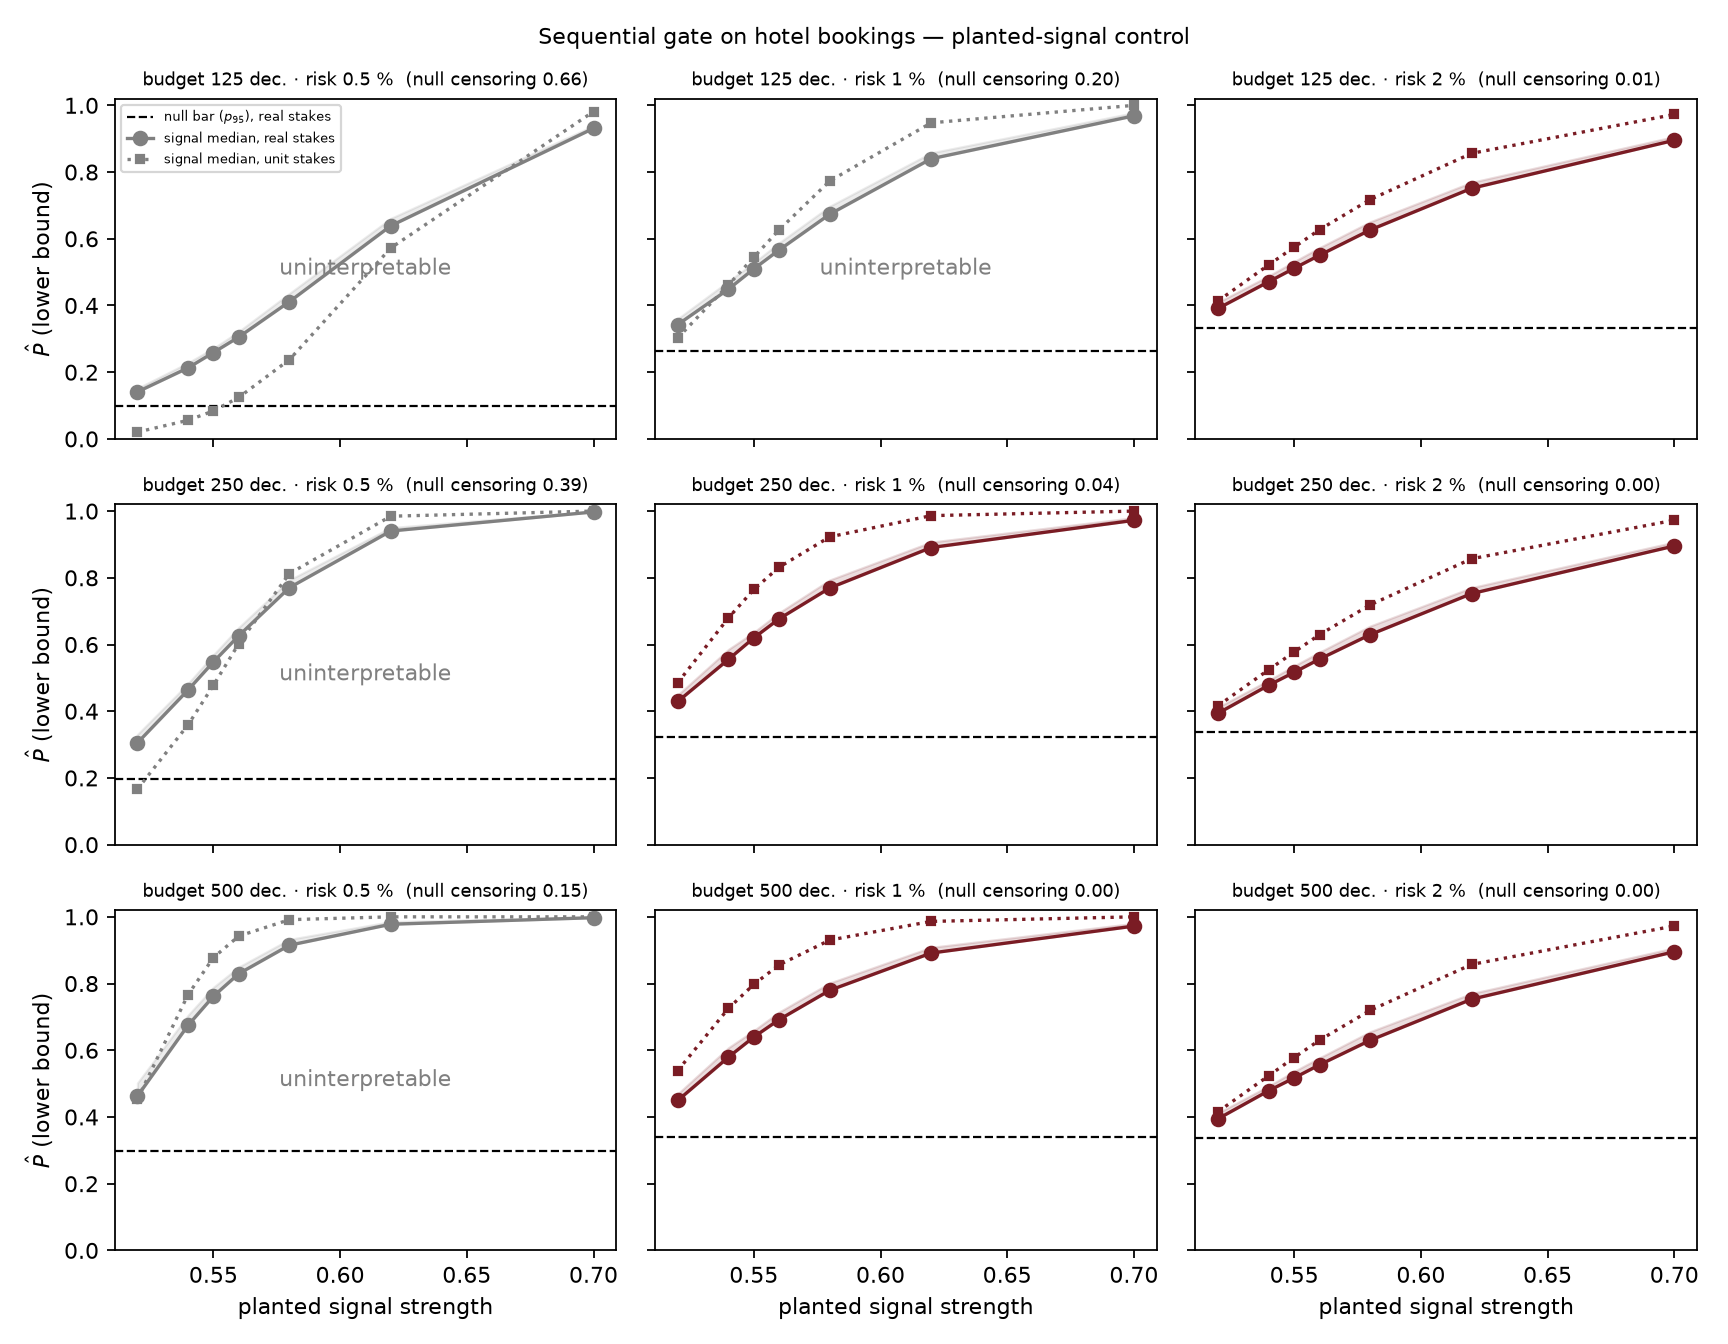
\includegraphics[width=\textwidth]{fig4_cellules_hf}
\caption{Hotel bookings, nine cells (rows: decision budget; columns: risk per decision). Circles: median $\Pf$ with real stakes; squares: with unit stakes; dashed: the null's bar with real stakes. Grey cells are uninterpretable. The low-risk column is silent for the same reason as in Figure~\ref{fig:cells}.}
\label{fig:hotelcells}
\end{figure}

\paragraph{Heavy-tailed stakes cost power, not size.}
Replacing every booking's value by the median leaves the null's bar practically unchanged (0.313 with unit stakes against 0.323 with real stakes, at a budget of 250 and 1\% risk) but raises the planted signal's median by up to 15 points (strength 0.55: 0.765 against 0.620; strength 0.58: 0.923 against 0.770). A few large losses bust paths that a homogeneous stake would have carried through. Heterogeneous payoffs therefore reduce the power of a sequential gate without increasing its false-positive rate --- a second reason, after sample size, why the financial pipeline with its varying barrier distances is less powerful than the stylised gate. At 0.5\% risk the heavy tail cuts censoring (0.39 with real stakes against 0.72 with unit stakes at a budget of 250) because a few large bookings let paths conclude.

\paragraph{Power as a function of sample size, without a regime confound.}
Keeping only the most recent 125, 250, 500, 770, 2,000, 5,000 and 20,000 usable starts of the booking stream, in the cell with a budget of 250 and 1\% risk, gives Table~\ref{tab:hoteln} and Figure~\ref{fig:hoteln}. The null's bar falls monotonically from 0.692 to 0.589, 0.477, 0.463, 0.441, 0.383 and 0.367, while the planted signal's median stays between 0.48 and 0.57 for strength 0.55. Strength 0.55 becomes detectable from 500 usable starts, 0.58 from 250, 0.62 from 125. The false NO-GO at small sample size is driven by the null's bar rising as the few available paths overlap, not by the signal weakening. This is the clean version of the left panel of Figure~\ref{fig:n}, and it shows what the regime obscures in the right panel.

\begin{table}[t]
\centering\small
\caption{Hotel bookings, campaign HF-C (budget 250 decisions, risk 1\%). Null bar and margins as a function of the number of usable starts; above 2,000 starts, one path in five or twenty is played to keep about 1,000 paths. Bold: positive margin.}
\label{tab:hoteln}
\begin{tabular}{lrrrrrrr}
\toprule
Usable starts & 125 & 250 & 500 & 770 & 2\,000 & 5\,000 & 20\,000 \\
\midrule
Paths played & 125 & 250 & 500 & 770 & 2\,000 & 1\,000 & 1\,000 \\
Null bar ($p_{95}$) & 0.692 & 0.589 & 0.477 & 0.463 & 0.441 & 0.383 & 0.367 \\
\midrule
Margin, $s=0.55$ & -0.212 & -0.037 & \textbf{+0.044} & \textbf{+0.061} & \textbf{+0.092} & \textbf{+0.139} & \textbf{+0.204} \\
Margin, $s=0.58$ & -0.068 & \textbf{+0.095} & \textbf{+0.173} & \textbf{+0.180} & \textbf{+0.214} & \textbf{+0.257} & \textbf{+0.336} \\
Margin, $s=0.62$ & \textbf{+0.124} & \textbf{+0.251} & \textbf{+0.319} & \textbf{+0.337} & \textbf{+0.343} & \textbf{+0.383} & \textbf{+0.455} \\
\bottomrule
\end{tabular}

\end{table}

\begin{figure}[t]
\centering
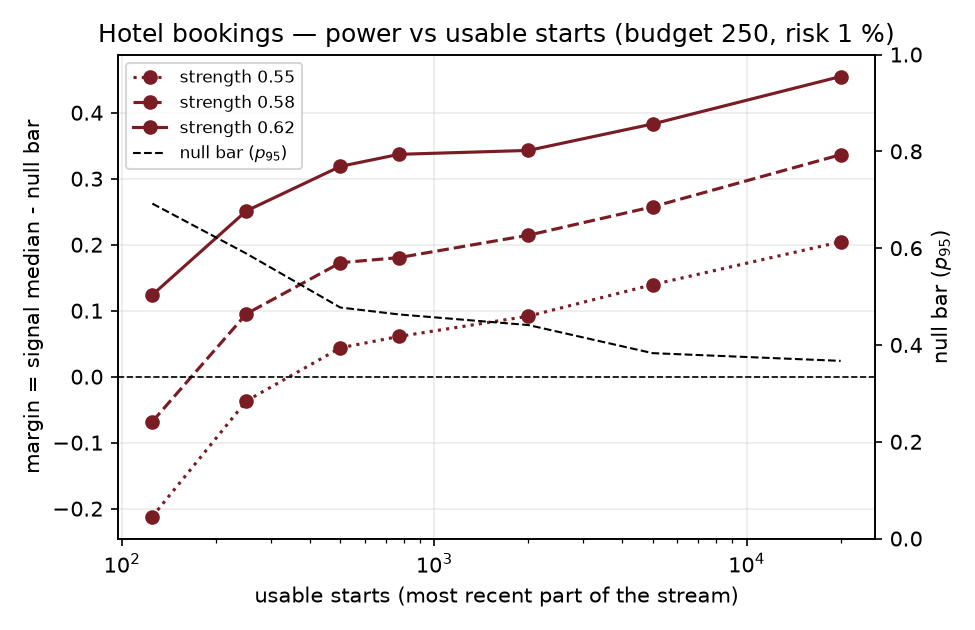
\includegraphics[width=0.75\textwidth]{fig5_puissance_n_hf}
\caption{Hotel bookings, campaign HF-C. Margin of three planted strengths (left axis) and the null's bar (right axis, dashed) as a function of usable starts, log scale.}
\label{fig:hoteln}
\end{figure}

\section{Three Ways to Get a Meaningless ``Detectable''}
\label{sec:guards}

The positive controls found three failure modes in the pipeline's own history, each of which produced a confident verdict with no content. We list them because each is generic.

\paragraph{A saturated grid.}
An early version of the control tested strengths 0.70 and 0.90, both of which returned $\Pf = 1.000$; the monotonicity proof compared 1.0 to 1.0 and passed, and the ``smallest detectable strength'' could only return the smallest value on the grid. The true floor, with the pipeline's settings of the time, was 0.60. A positive control must include strengths that the pipeline fails to see, or it proves nothing even when it passes. Our grids start at 0.52 for this reason.

\paragraph{A wrong chance reference.}
The chance accuracy of a coin-flip direction in this pipeline is not 50\%: the 2\% of labels that lose in both directions make it $(n_{\uparrow} + n_{\downarrow}) / (2 n_{\text{decided}}) \approx 48.3\%$, where $n_{\text{decided}}$ counts the labels that did not time out. A reference of 49.7\% had been written as a constant in an earlier evaluation; every candidate's lift was understated by about one standard error, always in the same direction. The reference of a null must be recomputed on the selection the candidate actually traded, never stored.

\paragraph{An uncensored null.}
Section~\ref{sec:uninterp} describes the bar of 0.001 produced by a null whose paths almost never concluded. The censoring guard is now a precondition of the verdict, not a figure printed beside it. The general rule: a lower bound that counts censored paths as failures is only a bound on the signal if the censoring rate is low for both the signal and the null.

\section{Limitations}
\label{sec:limits}

One market, one labelling, one scheduler, one sizing rule and one set of evaluation rules were tested; the numbers are specific to this pipeline, and the paper's claim is about the \emph{shape} of its power, not about its values transferring. The planted signal is a perfect model on a hidden variable (the realized label), so it measures the power of the evaluation chain given a decider of known accuracy; it does not measure whether a learner can reach that accuracy from features. Sixty direction seeds per cell is enough to see one-to-seven-point noise in the bar, not to estimate it precisely. Transaction costs are not modelled, and would lower every $\Pf$ including the null's. On the single market series, sample size and regime are confounded (Section~\ref{sec:n}); the hotel stream shows the clean curve, but hotel bookings have their own seasonality. Two reading conventions are fixed rather than derived: the 10\% censoring threshold, and the ``clear'' criterion of one standard deviation of the bar, which is deliberately lenient. The sealed hold-out was never opened, so nothing here says whether the NASDAQ series contains a tradable signal.

\section{Conclusion}
\label{sec:conclusion}

A validation pipeline is a measuring instrument, and an instrument has a sensitivity. We measured the sensitivity of a complete backtest-to-verdict pipeline by planting directional signals of known strength and found that it is not a constant: on the same data and the same code, the smallest detectable signal ranges from a 54\% to a 58\% directional accuracy across operating cells, five of nine cells cannot be read at all, doubling the risk budget turns a 70\% signal from a certain pass into a two-in-three pass, and a single null draw moves the bar by up to seven points. Shortening the history shows the mechanism of the false NO-GO: the null's bar rises when few overlapping paths are available while the true signal's median does not fall, so a weak true signal is rejected for lack of sample. A sequential gate on hotel bookings reproduces the censoring, risk and sample-size patterns and adds one: heavy-tailed stakes cost power without creating false positives.

The practical recommendation is short. A pipeline that reports ``no signal'' should report, next to it, the smallest planted signal it would have detected in the same cell, the censoring rate of its null, and the noise of its bar. Without these three numbers a NO-GO is indistinguishable from a pipeline that could not have said GO.

\paragraph{Reproducibility.}
The code of the pipeline, the positive-control module and its proof suite, the campaign drivers, every dated output file (\texttt{points.csv}, \texttt{meta.json} with grid and commit hash) and the scripts that generate every table and figure of this paper from those files are released at \url{https://github.com/hugomarotin-git/ml-papers}, folder \texttt{paper1-backtest-power}. The hotel dataset is public \citep{antonio2019}.

\bibliographystyle{plainnat}
\bibliography{references}
\end{document}
